\documentclass[aspectratio=169,12pt]{beamer}

\usepackage[T2A]{fontenc}
\usepackage[utf8]{inputenc}
\usepackage[russian]{babel}
\usepackage{amsmath, amssymb}
\usepackage{booktabs}
\usepackage{graphicx}
\usepackage{hyperref}

\newcommand{\rub}{~руб.}

\usetheme{CambridgeUS}
\usecolortheme{lily}
\setbeamertemplate{navigation symbols}{}
\setbeamertemplate{footline}[frame number]

\title{Прогноз цены смартфонов на Авито}
\date{}


\graphicspath{{figures/}}

\begin{document}

% ------------------------------------------------------------------
\begin{frame}
  \titlepage
\end{frame}

% ------------------------------------------------------------------
\begin{frame}{Содержание}
  \tableofcontents
\end{frame}

% ==================================================================
\section{Постановка задачи}

\begin{frame}{Цель и мотивация}
  \textbf{Задача:} по тексту и атрибутам объявления предсказать цену смартфона.

  \vspace{0.6em}
  \textbf{Зачем:}
  \begin{itemize}
    \item оценка «рыночной» цены для покупателя/продавца;
    \item выявление аномально дорогих или дешёвых предложений;
  \end{itemize}

  \vspace{0.6em}
  \textbf{Целевая переменная:} цена объявления, \rub \\

    \vspace{0.6em}
  \textbf{Оценка ошибки:} MAPE \\
\end{frame}

\begin{frame}{Данные}
  \begin{itemize}
    \item \textbf{Источник:} Авито, категория «Мобильные телефоны», Санкт-Петербург
    \item \textbf{Период:} последние 14 дней
    \item \textbf{Объём:} $\approx 7800$ объявлений
    \item \textbf{Фильтр цен:} от 500 до 200\,000 \rub
  \end{itemize}

  Данные были собраны с помощью парсера, который обходит страницы и сохраняет ключевые поля.

  \vspace{0.5em}
  \begin{block}{Ограничения выборки}
    Сильный перекос в сторону Samsung ($\sim$78\%) и Apple ($\sim$14\%).
    Модель в первую очередь описывает массовый сегмент рынка.
  \end{block}
\end{frame}

% ==================================================================
\section{Сбор и подготовка данных}

\begin{frame}{Парсинг Авито}
  \textbf{Инструменты:} Готовый парсер из открытых источников
  
  \textbf{Ключевые поля:}
  \begin{itemize}
    \item Название
    \item Цена
    \item Описание
    \item Дата публикации
    \item Адрес (район)
    \item «Поднято» (используется ли платное продвижение)
    \item Изображения (кол-во фотографий)
  \end{itemize}
  \vspace{0.5em}
\end{frame}

\begin{frame}{EDA}
  \begin{minipage}{0.48\textwidth}
    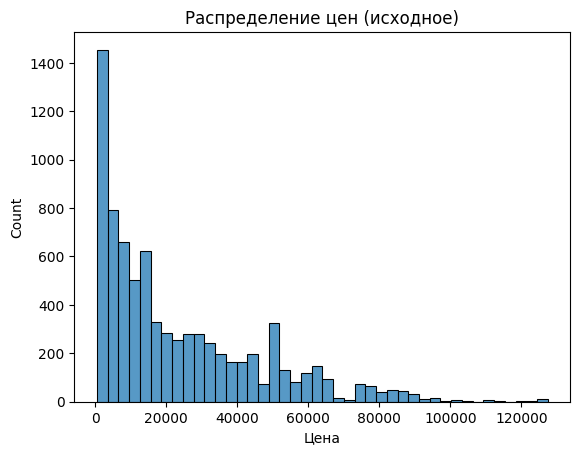
\includegraphics[width=\linewidth]{prices_raw.png}
    Сильный перекос в сторону недорогих моделей, длинный хвост дорогих.
  \end{minipage}\hfill
  \begin{minipage}{0.48\textwidth}
    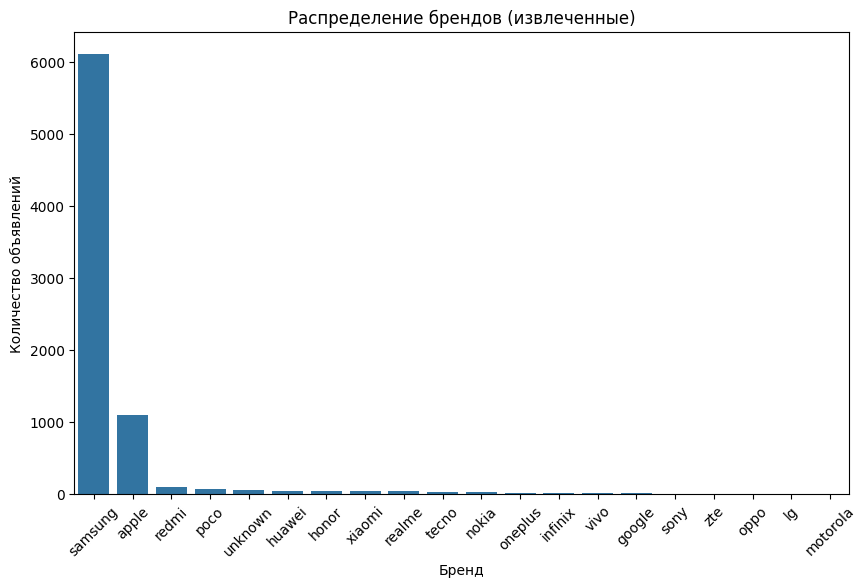
\includegraphics[width=\linewidth]{brands.png}
    Доминируют Samsung и Apple, остальные бренды представлены слабо.
  \end{minipage}
\end{frame}

\begin{frame}{EDA}
  \begin{minipage}{0.48\textwidth}
    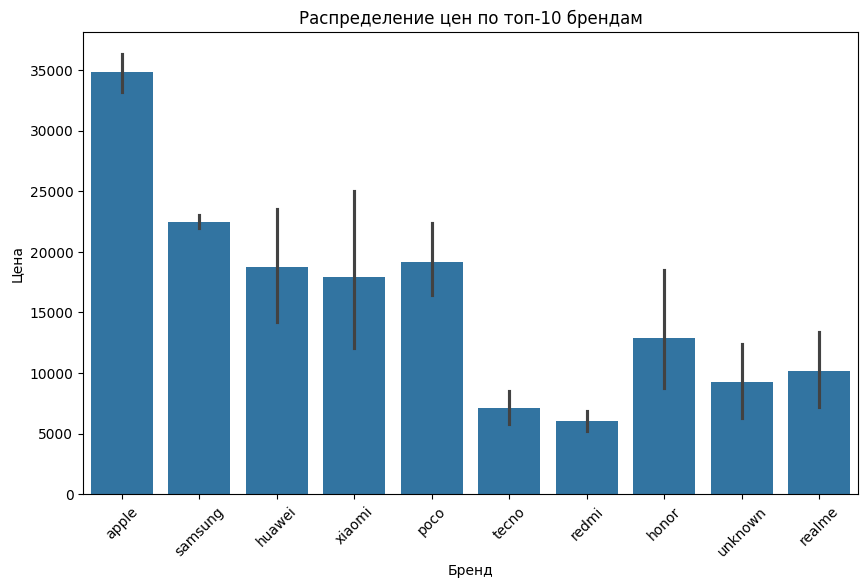
\includegraphics[width=\linewidth]{prices_by_brand.png}
    Цены по брендам: Apple дороже, Samsung дешевле, остальные еще дешевле.
  \end{minipage}\hfill
  \begin{minipage}{0.48\textwidth}
    % \includegraphics[width=\linewidth]{promoted.png}
    Примерно 20\% объявлений с платным продвижением, они в среднем дороже.
  \end{minipage}
\end{frame}

% ==================================================================
\section{Признаки}

\begin{frame}{Feature engineering}
  \small
  \begin{table}
    \centering
    \begin{tabular}{@{}ll@{}}
      \toprule
      \textbf{Источник} & \textbf{Новые признаки} \\
      \midrule
      Из «Название» & \texttt{brand}, \texttt{ram\_gb}, \texttt{storage\_gb}, \texttt{iphone\_gen}, флаги Pro/Max/Mini/Plus \\
      Из «Описание» & \texttt{has\_warranty}, \texttt{has\_box}, \texttt{has\_charger}, \texttt{condition} \\
      Метаданные & \texttt{is\_promoted}, \texttt{photos\_count}, \texttt{district}, \texttt{days\_since\_posted} \\
      Описание & \texttt{title\_only} $\rightarrow$ TF-IDF (300--800 признаков) \\
      \bottomrule
    \end{tabular}
  \end{table}

\end{frame}


\begin{frame}{Feature engineering}
  \begin{minipage}{0.65\textwidth}
    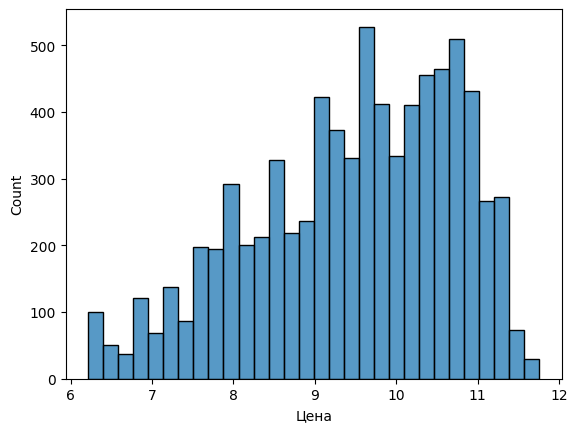
\includegraphics[width=\linewidth]{prices_log1p.png}
  \end{minipage}\hfill
  \begin{minipage}{0.35\textwidth}
    К признаку цены применено $\log(1 + y)$ для сглаживания хвоста и улучшения обучения моделей.
  \end{minipage}
\end{frame}


\begin{frame}{Итоговый набор признаков}
  \small
  \begin{table}
    \centering
\begin{tabular}{@{}lp{0.62\textwidth}@{}}
  \toprule
  \textbf{Тип признака} & \textbf{Названия признаков} \\
  \midrule
  Численные (16 шт.) &
    \texttt{ram\_gb}, \texttt{storage\_gb}, \texttt{iphone\_gen},
    \texttt{photos\_count}, \texttt{title\_len}, \texttt{description\_len},
    \texttt{days\_since\_posted}, \texttt{is\_pro}, \texttt{is\_max},
    \texttt{is\_mini}, \texttt{is\_plus}, \texttt{is\_promoted},
    \texttt{has\_warranty}, \texttt{has\_trade\_in}, \texttt{has\_box},
    \texttt{has\_charger}. \\
  Категориальные (3 шт.) &
    \texttt{brand}, \texttt{condition}, \texttt{district}. \\
  Текстовые &
    TF-IDF по \texttt{title\_only}, 300--800 признаков. \\
  \bottomrule
\end{tabular}
  \end{table}

\end{frame}


\begin{frame}{EDA новых признаков}
  \begin{minipage}{0.48\textwidth}
    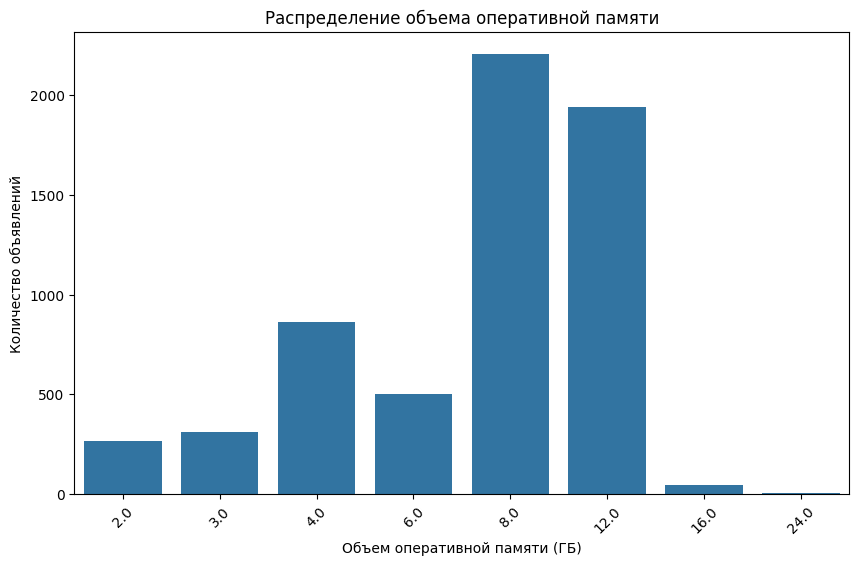
\includegraphics[width=\linewidth]{ram_dist.png}
    Наиболее популярные опции -- 8 и 12 ГБ
  \end{minipage}\hfill
  \begin{minipage}{0.48\textwidth}
    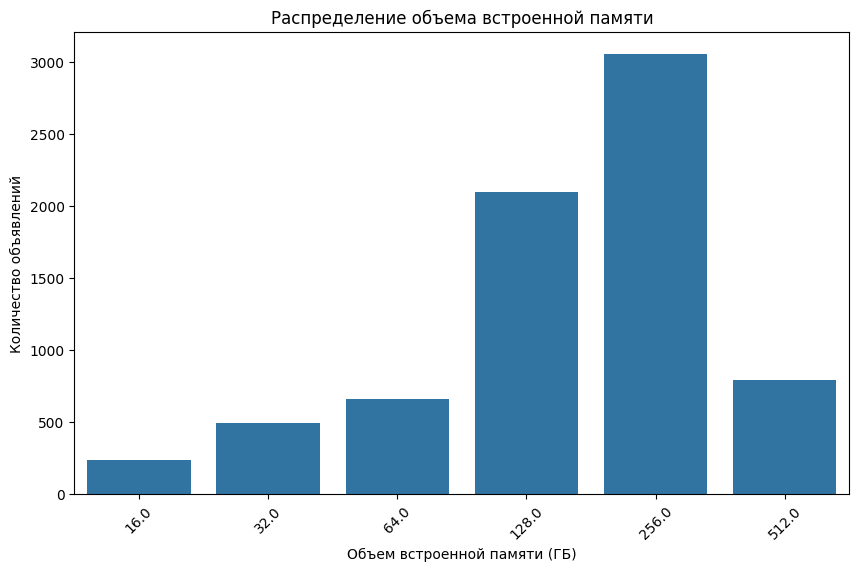
\includegraphics[width=\linewidth]{rom_dist.png}
    Преобладают 128 и 256 ГБ
  \end{minipage}
\end{frame}

\begin{frame}{EDA новых признаков}
  \begin{minipage}{0.48\textwidth}
    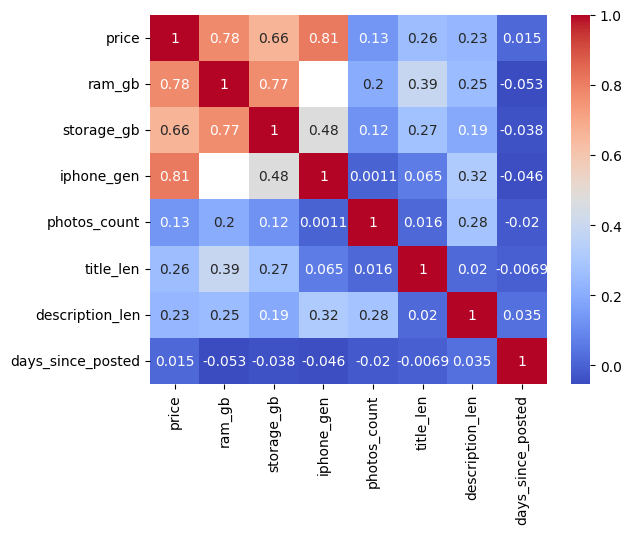
\includegraphics[width=\linewidth]{heatmap1.png}
  \end{minipage}\hfill
  \begin{minipage}{0.48\textwidth}
    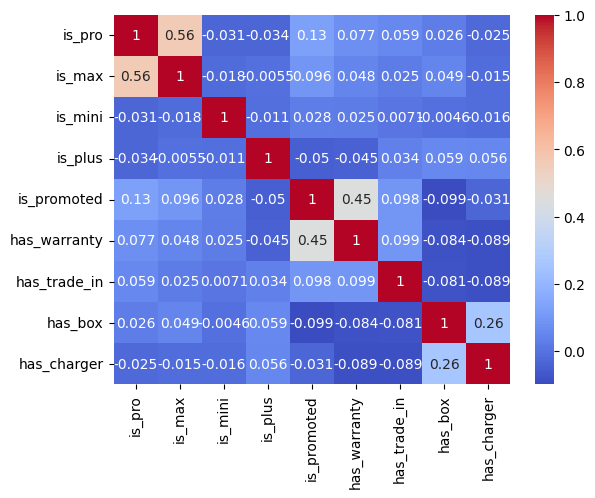
\includegraphics[width=\linewidth]{heatmap2.png}
  \end{minipage}
  Корреляций между числовыми признаками почти нет за исключением \texttt{ram\_gb} и \texttt{storage\_gb}, а также между флагом \texttt{is\_max}.
\end{frame}





\begin{frame}{TF-IDF}
    \begin{minipage}{0.48\textwidth}
      % show image if present, otherwise a placeholder box
    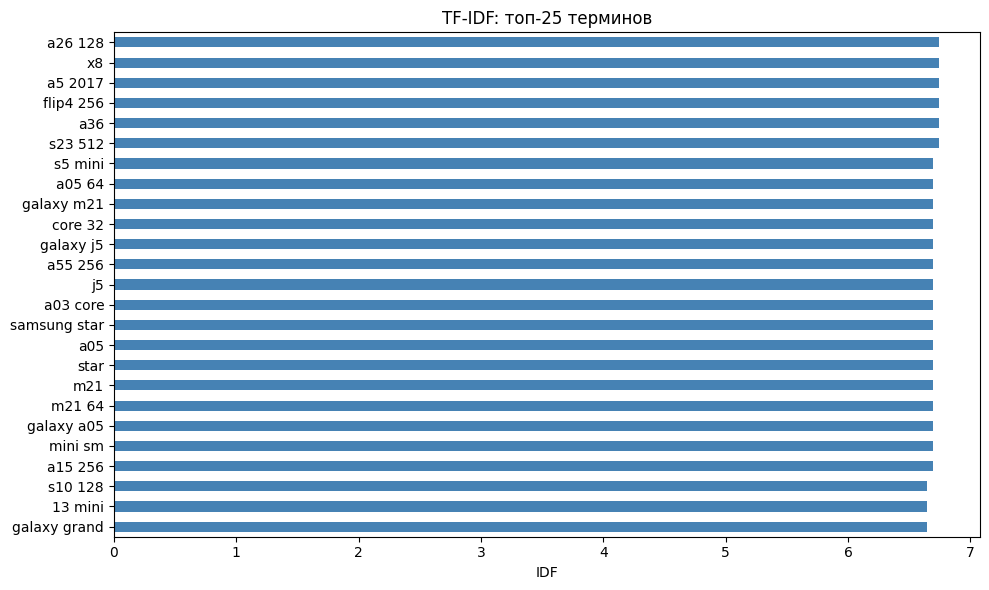
\includegraphics[width=\linewidth]{tfidf.png}
    \end{minipage}\hfill
    \begin{minipage}{0.48\textwidth}
        TF-IDF по названию позволяет выделить важные слова, связанные с ценой (например, «13 mini», «s10 128», «flip4 256»).
    \end{minipage}
\end{frame}

% ==================================================================
\section{Модели}

\begin{frame}{Сравниваемые модели}
  \begin{table}
    \centering
    \small
    \begin{tabular}{@{}ll@{}}
      \toprule
      \textbf{Модель} & \textbf{Комментарий} \\
      \midrule
      Dummy (mean) & baseline \\
      Ridge & применяется StandardScaler \\
      Decision Tree & ограничение 14 уровней \\
      Random Forest & 200 деревьев, 12 уровней \\
      CatBoost & 800 деревьев, depth 6, learning\_rate 0.05 \\
      LightGBM & $<$1500 деревьев, num\_leaves 31, subsample 0.85 \\
      \bottomrule
    \end{tabular}
  \end{table}

  \vspace{0.5em}
  Разделение выборки: 80\% train, 20\% test. \\
\end{frame}

% ==================================================================
\section{Результаты}

\begin{frame}{Метрики на всей тестовой выборке}
  % TODO: подставьте числа из test_notebook или artifacts/metrics_*.json
  \begin{table}
    \centering
    \begin{tabular}{@{}lrrr@{}}
      \toprule
      \textbf{Модель} & \textbf{MAPE} & \textbf{MAE, \rub} & \textbf{RMSE, \rub} \\
      \midrule
      Dummy & \textit{207\%} & \textit{17712} & \textit{25450} \\
      Ridge & \textit{22.8\%} & \textit{3230} & \textit{5452} \\
      Decision Tree & \textit{24.0\%} & \textit{2929} & \textit{5833} \\
      Random Forest & \textit{25.1\%} & \textit{3187} & \textit{5948} \\
      CatBoost & \textit{20.3\%} & \textit{2813} & \textit{4717} \\
      LightGBM & \textit{9.1\%} & \textit{1213} & \textit{2850} \\
      \bottomrule
    \end{tabular}
  \end{table}

  \vspace{0.5em}
  \textbf{Лучшая модель:} \textit{LightGBM} \\
\end{frame}


\begin{frame}{MAPE по сегментам тестовой выборки}
  \footnotesize
  \centering
  \begin{tabular}{@{}lrrr@{}}
    \toprule
    \textbf{Модель} & \textbf{Apple} & \textbf{Samsung} & \textbf{Остальные} \\
    & \multicolumn{1}{c}{\scriptsize $n{=}236$} &
      \multicolumn{1}{c}{\scriptsize $n{=}1191$} &
      \multicolumn{1}{c}{\scriptsize $n{=}132$} \\
    \midrule
    Dummy & 62.1\% & 227.1\% & 285.1\% \\
    Ridge & 24.1\% & 20.0\% & 46.5\% \\
    Decision Tree & 18.4\% & 18.9\% & 80.3\% \\
    Random Forest & 21.5\% & 21.9\% & 59.9\% \\
    CatBoost & 21.3\% & 16.6\% & 52.1\% \\
    \textbf{LightGBM} & \textbf{14.7\%} & \textbf{4.6\%} & \textbf{39.3\%} \\
    \bottomrule
  \end{tabular}

  \vspace{0.6em}
  \small
  Практически все модели дают лучший результат на сегменте Samsung, так как данных по нему больше всего.
\end{frame}

\begin{frame}{Метрики по сегментам: Apple и Samsung}
  \scriptsize
  \begin{columns}[T]
    \column{0.49\textwidth}
    \centering
    \textbf{Apple (iPhone)}, $n=236$
    \vspace{0.3em}

    \begin{tabular}{@{}lrrr@{}}
      \toprule
      \textbf{Модель} & \textbf{MAPE} & \textbf{MAE, \rub} & \textbf{RMSE, \rub} \\
      \midrule
      Dummy & 62.1\% & 26158 & 36160 \\
      Ridge & 24.1\% & 4675 & 7320 \\
      Decision Tree & 18.4\% & 4995 & 8461 \\
      Random Forest & 21.5\% & 5577 & 9090 \\
      CatBoost & 21.3\% & 4298 & 6773 \\
      LightGBM & 14.7\% & 2873 & 5149 \\
      \bottomrule
    \end{tabular}

    \column{0.49\textwidth}
    \centering
    \textbf{Samsung}, $n=1191$
    \vspace{0.3em}

    \begin{tabular}{@{}lrrr@{}}
      \toprule
      \textbf{Модель} & \textbf{MAPE} & \textbf{MAE, \rub} & \textbf{RMSE, \rub} \\
      \midrule
      Dummy & 227.1\% & 16852 & 23833 \\
      Ridge & 20.0\% & 2893 & 4853 \\
      Decision Tree & 18.9\% & 2215 & 4448 \\
      Random Forest & 21.9\% & 2523 & 4617 \\
      CatBoost & 16.6\% & 2379 & 3833 \\
      LightGBM & 4.6\% & 688 & 1413 \\
      \bottomrule
    \end{tabular}
  \end{columns}

  \vspace{0.4em}
\end{frame}

\begin{frame}{Метрики по сегментам: остальные бренды}
  \footnotesize
  \centering
  \textbf{Остальные} (не Apple и не Samsung), $n=132$

  \vspace{0.5em}
  \begin{tabular}{@{}lrrr@{}}
    \toprule
    \textbf{Модель} & \textbf{MAPE} & \textbf{MAE, \rub} & \textbf{RMSE, \rub} \\
    \midrule
    Dummy & 285.1\% & 10369 & 13683 \\
    Ridge & 46.5\% & 3685 & 6541 \\
    Decision Tree & 80.3\% & 5676 & 9766 \\
    Random Forest & 59.9\% & 4907 & 8819 \\
    CatBoost & 52.1\% & 4077 & 6944 \\
    LightGBM & 39.3\% & 2984 & 5524 \\
    \bottomrule
  \end{tabular}

  \vspace{0.6em}
  \small
  Мало примеров в test $\Rightarrow$ высокий разброс; деревья переобучаются сильнее бустинга.
\end{frame}


\begin{frame}{Качество предсказаний}
  \centering
  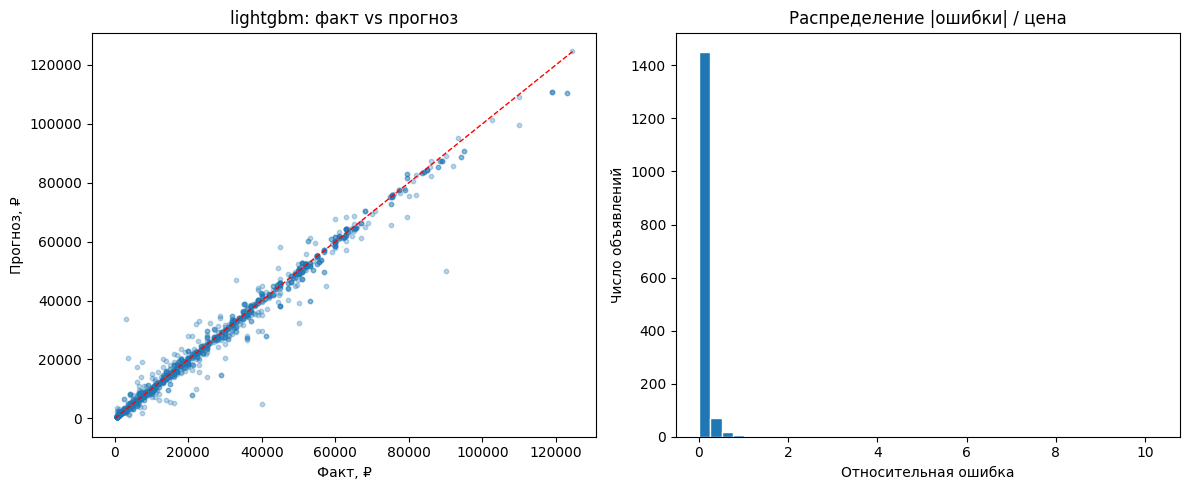
\includegraphics[width=0.9\linewidth]{results.png}
 
\end{frame}

\begin{frame}{Качество предсказаний}
  \centering
  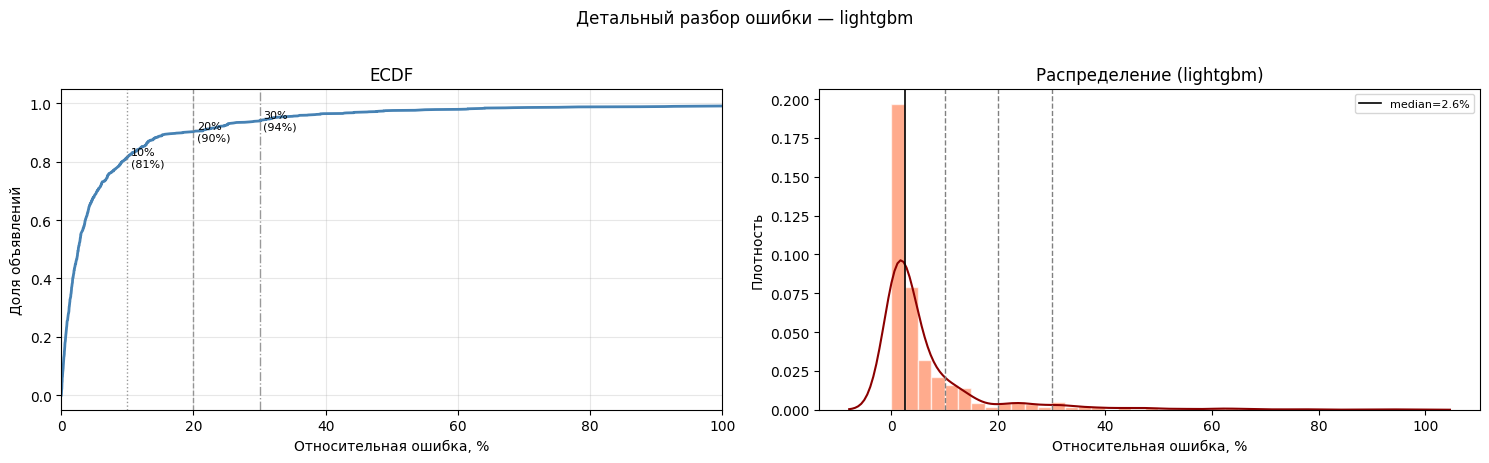
\includegraphics[width=0.9\linewidth]{error_stats.png}
 
\end{frame}

\begin{frame}{Пример объявления}
  \footnotesize
  \begin{columns}[T]
    \column{0.48\textwidth}
    \textbf{Название:} iPhone 15 Pro, 512 ГБ, SIM + eSIM

    \vspace{0.4em}
    \begin{itemize}
      \item \textbf{Бренд:} Apple
      \item \textbf{Память:} 512 ГБ
      \item \textbf{Описание:} В идеальном состоянии, носила только в чехлах, не падал, ничего не ломалось. Отдам 2 чехла.
Без Торга, обмена на нокию с доплатой и прочего.
      \item \textbf{Цена (факт):} 52\,000 \rub
    \end{itemize}

    \vspace{0.3em}
    \scriptsize
    CatBoost ближе всего к факту (ошибка 4.1\%).

    \column{0.50\textwidth}
    \centering
    \begin{tabular}{@{}lrrr@{}}
      \toprule
      \textbf{Модель} & \textbf{Прогноз} & \textbf{Ошибка} & \textbf{\%} \\
      \midrule
      CatBoost & 49\,890 & 2\,110 & 4.1\% \\
      LightGBM & 55\,831 & 3\,831 & 7.4\% \\
      Random Forest & 48\,026 & 3\,974 & 7.6\% \\
      Decision Tree & 56\,202 & 4\,202 & 8.1\% \\
      Ridge & 43\,994 & 8\,006 & 15.4\% \\
      Dummy & 12\,891 & 39\,109 & 75.2\% \\
      \midrule
      \textbf{Факт} & \multicolumn{3}{c}{\textbf{52\,000 \rub}} \\
      \bottomrule
    \end{tabular}
  \end{columns}
\end{frame}

% ==================================================================
\section{Выводы}

\begin{frame}{Выводы и ограничения}
  \textbf{Выводы:}
  \begin{itemize}
    \item собран датасет из 7793 объявлений;
    \item бустинг (CatBoost/LightGBM) превосходит линейные модели и dummy;
    \item TF-IDF названия и \texttt{brand} --- ключевые сигналы цены.
  \end{itemize}

  \vspace{0.5em}
  \textbf{Ограничения:}
  \begin{itemize}
    \item дисбаланс брендов, низкое качество данных по менее популярным брендам;
    \item признак \texttt{iphone\_gen} неинформативен вне Apple;
    \item парсинг усложняется из-за ограничений и блокировок со стороны Авито.
  \end{itemize}

  \vspace{0.5em}
  \textbf{Улучшения:} отдельные модели под каждый бренд, доработка сбора данных
\end{frame}

\begin{frame}
  \centering
  \Large Спасибо за внимание!

\end{frame}

\end{document}
